\documentclass[11pt,a4paper]{article}
\usepackage[utf8]{inputenc}
\usepackage[T1]{fontenc}
\usepackage[margin=2.3cm]{geometry}
\usepackage{graphicx}\usepackage{caption}\usepackage{booktabs}\usepackage{tabularx}
\usepackage{float}\usepackage[hidelinks]{hyperref}\usepackage{microtype}
\captionsetup{font=small,labelfont=bf}
\setlength{\parskip}{0.45em}\setlength{\parindent}{0pt}
\renewcommand{\arraystretch}{1.15}

\begin{document}
\begin{center}
{\large\bfseries Shadow: badminton drills at home, where the shuttle always flies}\\[0.25em]
{\small Giving the learner control of the coaching, not of the task}\\[0.6em]
{\small Atharva Waghmare \quad\textbar\quad AXW1008 \quad\textbar\quad Intelligent Interactive Systems, A2}\\[0.3em]
{\small\bfseries Total 1286 words} {\small(abstract 290 + main report 996; figures, captions and references excluded)}\\[0.2em]
{\small Repository: \url{https://github.com/AtharvaOnGitHub/VR-badminton-coach} \quad\textbar\quad submitted release: tag \texttt{a2-submission}}
\end{center}

\section*{Abstract}

A club player who wants to fix their smash between sessions has no good option.
Shadow swinging in a living room produces no outcome at all: you cannot see where the
shot would have gone, so there is nothing to learn from. Court time needs a partner and
a booking. Most practice happens with nobody watching and nothing to react to.

Shadow is a home trainer that supplies the missing half. The player stands in a full
virtual badminton hall with their own furniture fading in through passthrough as they
approach it. A drill feeder lifts a high clear; the player steps, swings, and the
shuttle leaves the racket on the trajectory their actual contact produced, clears the
net or does not, and lands in the target box or past it. That happens every rep,
because where the shuttle went is the task rather than an opinion about technique. A
jump smash wants about three metres of reach and a ceiling gives two, so the virtual
racket reaches 1.36 times further than the real one. That figure is shown, and
adjustable.

The coaching is the part that waits. After a block the system may offer one ignorable
line; the player can ask at any time, and what comes back names the reps it came from
and plots them against the reps that landed. Putting the same observation away twice
mutes it for the session, and a muted observation never returns on its own.

What is implemented is the drill loop, the flight model, the remap, the freeze, the
policy that decides whether to offer, and both player and coach surfaces. Head and
racket tracking are a labelled placeholder. Scope is one stroke, one session, one
player, with no retention measurement.

\section*{What it is, and who it is for}

The user is an intermediate club player with no regular coach, who knows their smash
is unreliable without knowing why. Taking a headset to the sports hall would be absurd;
this is for the evenings in between, in a living room cleared to roughly two arm-spans
by one.

Figures 1--3 show a rep: the feed with nothing overlaid on it, the same rep from the
side with the strike and the landing, and the freeze, where the dashed line is the gap
between where the shuttle is and where the stroke wants to meet it.

\section*{Design rationale}

\begin{table}[H]\small
\begin{tabularx}{\textwidth}{@{}p{3.3cm} X p{1.9cm}@{}}
\toprule
\textbf{Choice} & \textbf{Why it suits the problem, and the evidence} & \textbf{Status}\\
\midrule
The shuttle flies on every rep
& Two kinds of feedback get conflated. Where the shuttle landed is intrinsic to the task; a judgement about contact height is augmented, and only the second is what the retention literature warns about. Suppressing both leaves the player swinging at nothing, which is the problem they came with. Property four of the module's definition is a closed loop with a human, and with no outcome there is no loop.
& Implemented\\
\addlinespace
Full virtual hall, passthrough only for collision
& A shot needs somewhere to go; a passthrough living room has no net and no far court, so the outcome reads against nothing. Furniture fades in within 1.9 m, which is the one thing passthrough is genuinely needed for.
& Implemented\\
\addlinespace
Reach remap, 1.36$\times$, shown and adjustable
& Remapping maps a real movement onto a different virtual one; without it the stroke is impossible under a 2.4 m ceiling. It is shown and adjustable because a remap the player cannot see is not assistance but the system quietly changing the task, corrupting the mental model they build (L05).
& Implemented\\
\addlinespace
A feeder, not an opponent
& An opponent would train reaction and turn this into how realistically badminton can be played in a living room. A predictable feed keeps the stroke as the thing being trained.
& Implemented\\
\addlinespace
Coaching waits to be asked
& Who acts next is L01's first interaction variable. Horvitz's act/ask/wait (L03) weighs confidence against the cost of a poor guess: mid-rep the cost is high and the benefit unusable, so the system waits; between reps it may place one sentence the player can ignore.
& Implemented\\
\addlinespace
Two thresholds with hold times
& A single threshold has no memory, so a noisy signal makes the system flicker and a player cannot model it. Entry needs 0.60 across two blocks, release 0.35 across three: asymmetric because an unasked-for interruption must be earned, and because repeated false alarms erode response to later ones (signal detection and cry-wolf, L04).
& Implemented\\
\addlinespace
The player freezes; the system only offers
& Freezing mid-flight is the strongest teaching moment here, which is why the system does not take it. Agency is built from an intended action followed by the predicted result (Haggard, L06), so the commit stays the player's own. After three misses it offers; it never seizes.
& Implemented\\
\addlinespace
A three-step override ladder
& Easy dismissal and correction are Amershi G8 and G9, and a session-wide control is G17. A dismissal must not silently retrain anything (G14), so a mute never reverses itself when confidence rises.
& Implemented\\
\addlinespace
One observation, measured against your own good reps
& Working memory holds about four chunks (Cowan, L05), so a list of corrections cannot be acted on. Completeness drives accurate mental models while too little produces the belief that the system is guessing (Kulesza, L05), so the sentence names the reps it used and plots them against the ones that landed. Never against an expert: a single expert reference makes the judgement normative with no route to reject it, which A1 found to be the shared unexamined assumption of the systems reviewed.
& Implemented\\
\addlinespace
Coach surface behind approval
& Contracts are per action, by stakes and reversibility. Recording a rep is high-volume and reversible, so approval would collapse into reflex clicking; sharing cannot be undone, so it is the one action needing a deliberate act.
& Implemented\\
\addlinespace
LLM phrasing of observations
& Would improve the sentence without changing the decision, so it stays \emph{advise} and sits beside the loop. Cut: generated text cannot guarantee the evidence binding above.
& Planned\\
\bottomrule
\end{tabularx}
\end{table}

\section*{Architecture}

Figure 5 groups components by clock. Everything built is local, following the rule
that anything the body can feel must be: a swing is felt. The shuttle's flight sits on
the frame clock and is gated by nothing, because it is the task. The policy engine sits
on the block clock and decides only whether to \emph{offer}; it never gates what the
player pulls. No remote call exists, so a slow call that never returns has nothing to
handle, and the one planned remote component degrades to the template sentence.

Flight uses quadratic drag, not a parabola. A shuttle's terminal velocity is near
6.8 m/s, so it leaves the racket around 60 m/s and sheds almost all of it, which is
what gives badminton its shape.

\section*{What building it changed}

Three things only became visible by running it. An early flight model used 20 m/s
launch speeds and could not reach the net; the drag-to-mass ratio, not the geometry, was
wrong. Second, the contact-to-landing mapping was so sensitive that a centimetre of
timing moved the landing a quarter of a metre, which makes a drill feel random rather
than learnable; sweeping the model gave 18 degrees per metre and a 0.4 m window, about
220 ms. Third, the flight clock came from accumulated frame deltas, so wherever the
renderer was throttled the physics silently stopped and every rep reported an identical
contact. Time now comes from the wall clock. \texttt{tools/check.mjs} drives a real
browser and asserts all of this across nine checks.

\section*{Scope and honest limits}

Thresholds are defended by argument, not data from players. There is no retention
measurement, the outcome the underlying evidence turns on, and it cannot be established
inside this module. The swing is reduced to its timing, so the system models when
contact happened rather than how the arm got there. Mutes last one session.

\begin{figure}[H]\centering\includegraphics[width=0.80\textwidth]{fig/f1.png}
\caption{Mid-rep, first person. The shuttle is on its way and nothing is drawn over it.}\end{figure}

\begin{figure}[H]\centering\includegraphics[width=0.80\textwidth]{fig/f2.png}
\caption{The same rep from the side: the feeder's clear, the strike, and the landing
marker past the target box. This is the feedback the player gets on every rep.}\end{figure}

\begin{figure}[H]\centering\includegraphics[width=0.80\textwidth]{fig/f3.png}
\caption{The player has frozen the shuttle. Red is where it is, green is where the
stroke wants to meet it, and the dashed line is the gap.}\end{figure}

\begin{figure}[H]\centering\includegraphics[width=0.86\textwidth]{fig/f4.png}
\caption{The player asked. One sentence, the reps behind it, and every rep plotted so
the misses can be seen sitting below the ones that landed.}\end{figure}

\begin{figure}[H]\centering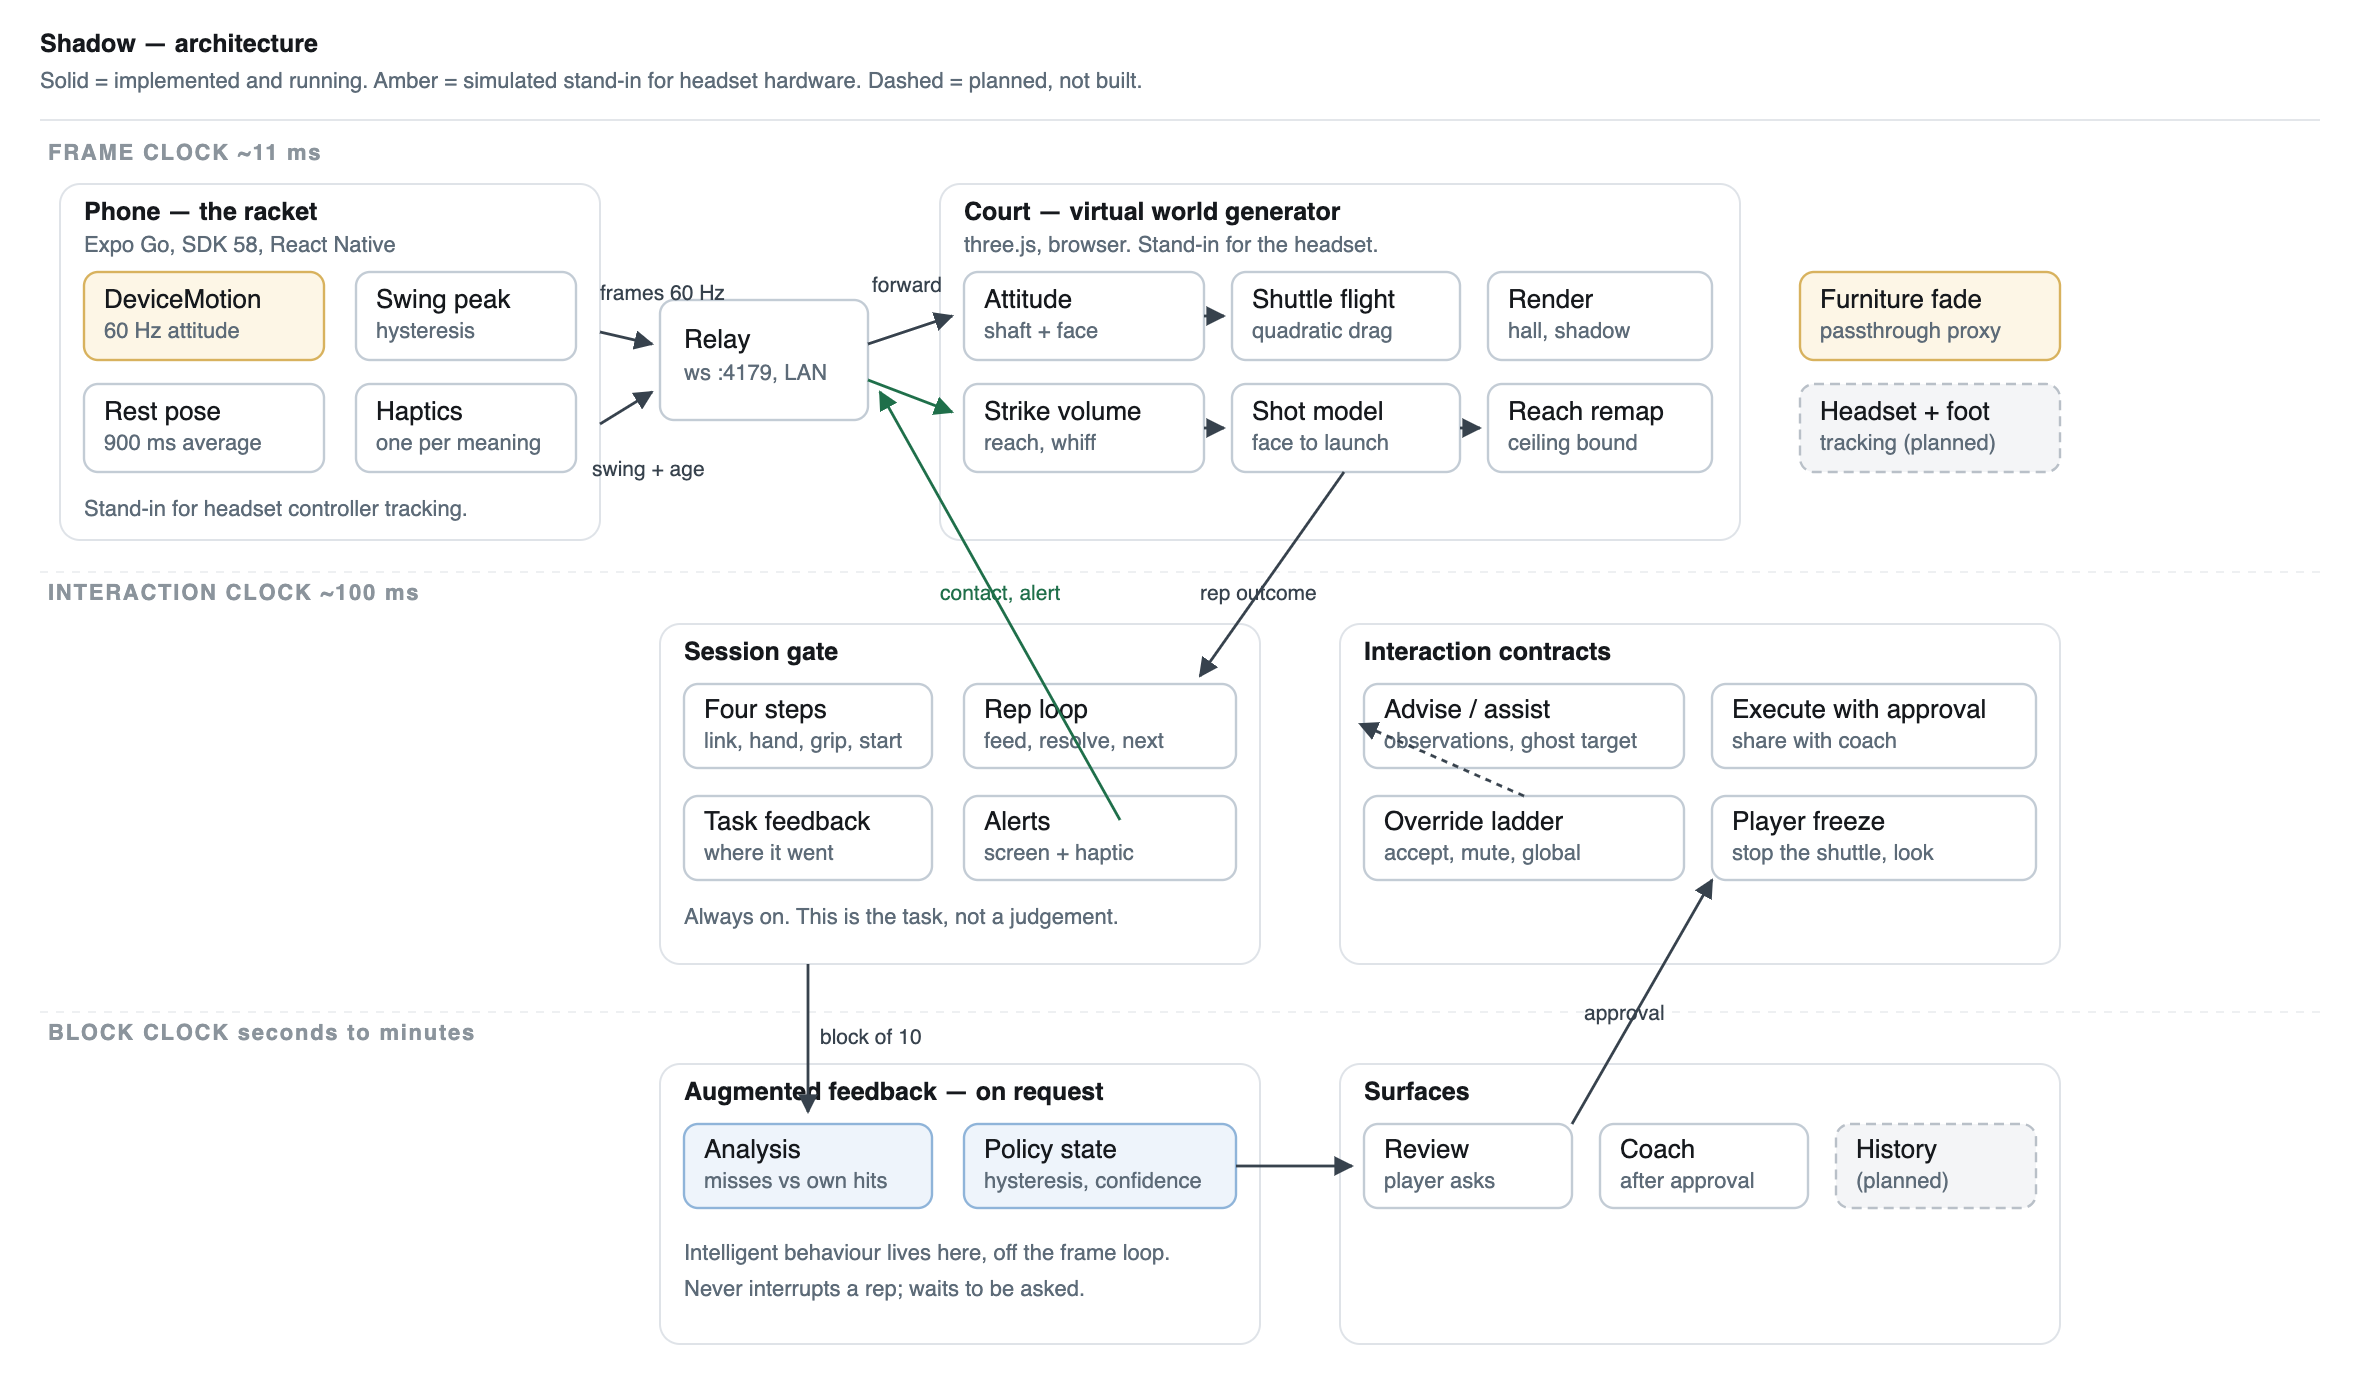
\includegraphics[width=\textwidth]{fig/architecture.png}
\caption{Components by clock, each marked implemented, simulated or planned, with the
contract on every action.}\end{figure}

\section*{References}
{\small
Amershi, S., Weld, D., Vorvoreanu, M., Fourney, A., Nushi, B., Collisson, P., Suh, J.,
Iqbal, S., Bennett, P. N., Inkpen, K., Teevan, J., Kikin-Gil, R., \& Horvitz, E. (2019).
Guidelines for human-AI interaction. \textit{CHI 2019}, Paper 3.

Cowan, N. (2001). The magical number 4 in short-term memory. \textit{Behavioral and
Brain Sciences}, 24(1), 87--114.

Haggard, P. (2017). Sense of agency in the human brain. \textit{Nature Reviews
Neuroscience}, 18(4), 196--207.

Horvitz, E. (1999). Principles of mixed-initiative user interfaces. \textit{CHI 1999},
159--166.

Kulesza, T., Stumpf, S., Burnett, M., Yang, S., Kwan, I., \& Wong, W.-K. (2013). Too
much, too little, or just right? Ways explanations impact end users' mental models.
\textit{IEEE VL/HCC 2013}, 3--10.

LaValle, S. M. (2023). \textit{Virtual Reality}. Cambridge University Press.

Norman, D. A. (2013). \textit{The Design of Everyday Things} (revised edition). Basic Books.

Sigrist, R., Rauter, G., Riener, R., \& Wolf, P. (2013). Augmented visual, auditory,
haptic, and multimodal feedback in motor learning: A review. \textit{Psychonomic
Bulletin \& Review}, 20, 21--53.
}
\end{document}
